\documentclass[10pt]{beamer}
\usepackage[english]{babel}
\usepackage[utf8]{inputenc}
\usepackage[T1]{fontenc}
\usepackage{helvet}
\usepackage{multicol}
%-------------------------------------------------------
% INFORMATION IN THE TITLE PAGE
%-------------------------------------------------------

\newcommand{\cstitle}{\textbf{Tópicos en Computación Gráfica}}
\subtitle[]{ArgosMol: A web tool for protein visualization}
\newcommand{\cscourseCode}{Tópicos en Computación Gráfica}
\newcommand{\csauthor}{MSc. Vicente Machaca Arceda}
\institute[UNSA]{Universidad Nacional de San Agustín}
\newcommand{\csemail}{vmachacaa@unsa.edu.pe}
\newcommand{\instituteabr}{UNSA}
\newcommand{\nameUp}{}
\date{2021}
\title[\cscourseCode]{\cstitle}
\author{\csauthor}
%%%%%%%%%%%%%%%%%

%-------------------------------------------------------
% CHOOSE THE THEME
%-------------------------------------------------------
\def\mycmd{0} % CS THEME
\def\mycmd{1} % MYTHEME
%-------------------------------------------------------

\if\mycmd1
	\usetheme[]{Feather}
	\newcommand{\chref}[2]{\href{#1}{{\usebeamercolor[bg]{Feather}#2}}}
\else
	\usepackage{csformat}
	\newcommand{\chref}[3][blue]{\href{#2}{\color{#1}{#3}}}%
\fi

\newcommand{\1}{
        	\setbeamertemplate{background}{
        		
\includegraphics[width=\paperwidth,height=\paperheight]{img/1}
        		\tikz[overlay] \fill[fill opacity=0.75,fill=white] (0,0) rectangle (-\paperwidth,\paperheight);
        	}
}



%-------------------------------------------------------
% THE BODY OF THE PRESENTATION
%-------------------------------------------------------

\begin{document}


\AtBeginSubsection[]
{
    \begin{frame}
        \frametitle{Overview}
        \tableofcontents[currentsubsection]
    \end{frame}
}


%-------------------------------------------------------
% THE TITLEPAGE
%-------------------------------------------------------

\if\mycmd1 % MY THEME
	\1{
	\begin{frame}[plain,noframenumbering] 
		\titlepage 
	\end{frame}}

\else % CS THEME
	\maketitle
\fi


%-------------------------------------------------------
%-------------------------------------------------------
\begin{frame}{Content}
	\tableofcontents
\end{frame}
%-------------------------------------------------------
%-------------------------------------------------------


%%%%%%%%%%%%%%%%%%%%%%%%%%%%%%%%%%%%%%%%%%%%%%%%%%%%%%%%%%%%%%%%%%%%%%%%%%%%%%%%%%%%%%%%%%%%%%%%%%%%%%%%%%%%%%%%
%%%%%%%%%%%%%%%%%%%%%%%%%%%%%%%%%%%%%%%%%%%%%%%%%%%%%%%%%%%%%%%%%%%%%%%%%%%%%%%%%%%%%%%%%%%%%%%%%%%%%%%%%%%%%%%%
%%%%%%%%%%%%%%%%%%%%%%%%%%%%%%%%%%%%%%%%%%%%%%%%%%%%%%%%%%%%%%%%%%%%%%%%%%%%%%%%%%%%%%%%%%%%%%%%%%%%%%%%%%%%%%%%
\section{Introduction}
%%%%%%%%%%%%%%%%%%%%%%%%%%%%%%%%%%%%%%%%%%%%%%%%%%%%%%%%%%%%%%%%%%%%%%%%%%%%%%%%%%%%%%%%%%%%%%%%%%%%%%%%%%%%%%%%
%%%%%%%%%%%%%%%%%%%%%%%%%%%%%%%%%%%%%%%%%%%%%%%%%%%%%%%%%%%%%%%%%%%%%%%%%%%%%%%%%%%%%%%%%%%%%%%%%%%%%%%%%%%%%%%%
%%%%%%%%%%%%%%%%%%%%%%%%%%%%%%%%%%%%%%%%%%%%%%%%%%%%%%%%%%%%%%%%%%%%%%%%%%%%%%%%%%%%%%%%%%%%%%%%%%%%%%%%%%%%%%%%

%%%%%%%%%%%%%%%%%%%%%%%%%%%%%%%%%%%%%%%%%%%%%%%%%%%%%%%%%%%%%%%%%%%%%%%%%%%%%%%%%%%%%%%%%%%%%%%%%%%%%%%%%%%%%%%%
%%%%%%%%%%%%%%%%%%%%%%%%%%%%%%%%%%%%%%%%%%%%%%%%%%%%%%%%%%%%%%%%%%%%%%%%%%%%%%%%%%%%%%%%%%%%%%%%%%%%%%%%%%%%%%%%
%%%%%%%%%%%%%%%%%%%%%%%%%%%%%%%%%%%%%%%%%%%%%%%%%%%%%%%%%%%%%%%%%%%%%%%%%%%%%%%%%%%%%%%%%%%%%%%%%%%%%%%%%%%%%%%%
\subsection{Definitions}
%%%%%%%%%%%%%%%%%%%%%%%%%%%%%%%%%%%%%%%%%%%%%%%%%%%%%%%%%%%%%%%%%%%%%%%%%%%%%%%%%%%%%%%%%%%%%%%%%%%%%%%%%%%%%%%%
%%%%%%%%%%%%%%%%%%%%%%%%%%%%%%%%%%%%%%%%%%%%%%%%%%%%%%%%%%%%%%%%%%%%%%%%%%%%%%%%%%%%%%%%%%%%%%%%%%%%%%%%%%%%%%%%
%%%%%%%%%%%%%%%%%%%%%%%%%%%%%%%%%%%%%%%%%%%%%%%%%%%%%%%%%%%%%%%%%%%%%%%%%%%%%%%%%%%%%%%%%%%%%%%%%%%%%%%%%%%%%%%%

%-------------------------------------------------------
%-------------------------------------------------------
\begin{frame}{Definitions}{}	
	
	\begin{columns}
		\begin{column}{0.48\textwidth}
			
			\begin{block}{}
				\textbf{Proteomics} is the large-scale study of proteins \cite{anderson1998proteome}
			\end{block}
		
			\begin{block}{}
				\textbf{Proteins} are large, complex molecules that play many critical roles in the body. They do most of the work in cells. \cite{anderson1998proteome}
			\end{block}

		\end{column}
	
		\begin{column}{0.48\textwidth}
		
			\begin{figure}
				\centering
				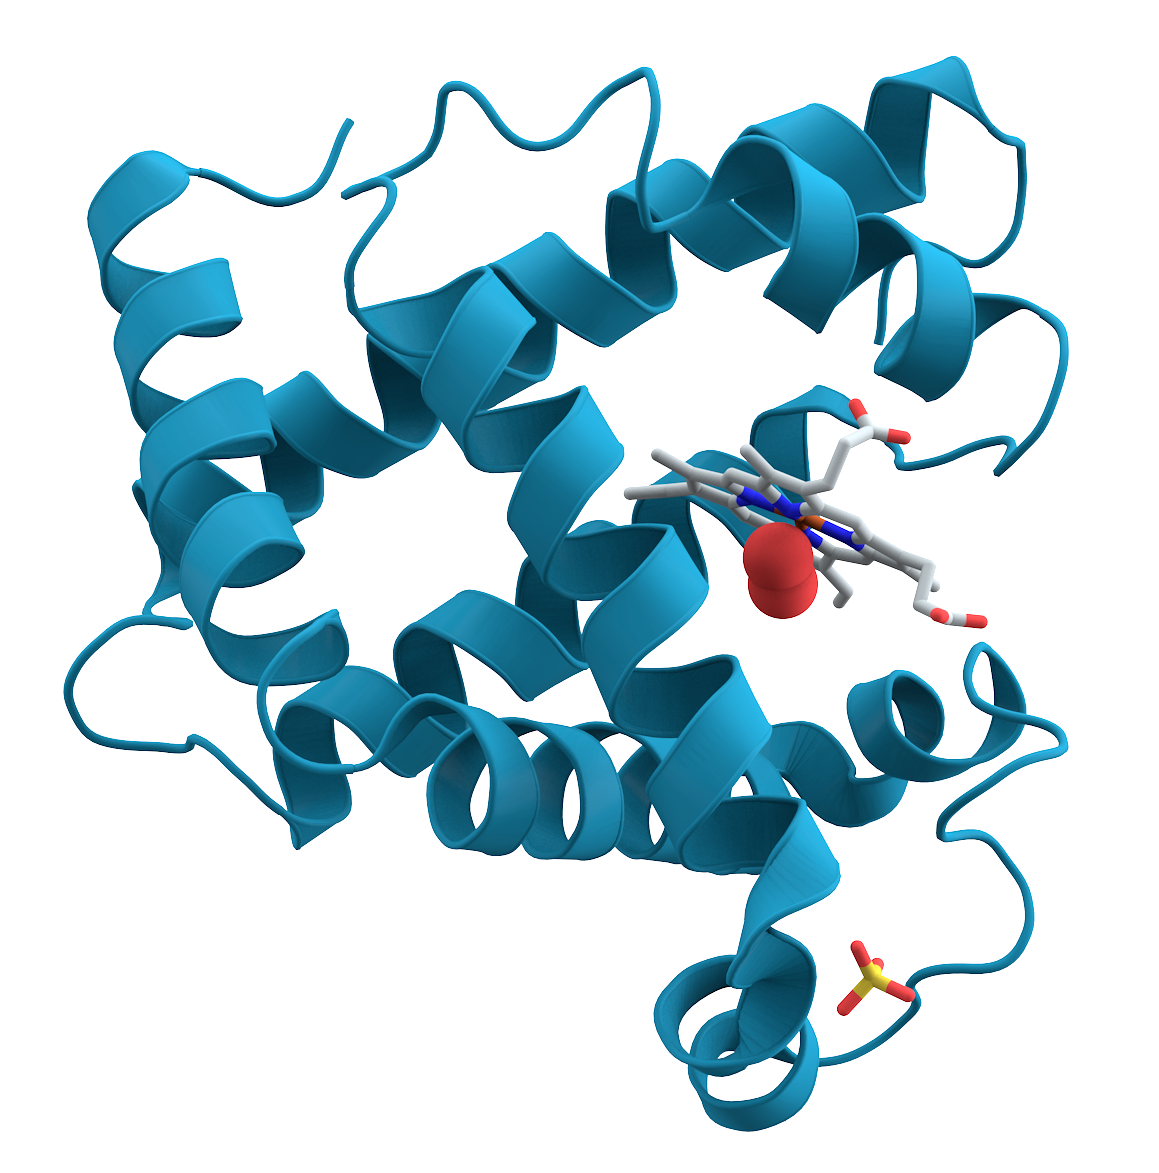
\includegraphics[width=5cm]{img/papers/myoglobin}
				\caption{A representation of the 3D structure of the protein myoglobin. Source: \chref{https://pdb101.rcsb.org/motm/1}{PDB}.}
			\end{figure}	
		
		\end{column}
	\end{columns}	
		
\end{frame}
%-------------------------------------------------------
%-------------------------------------------------------

%-------------------------------------------------------
%-------------------------------------------------------
\begin{frame}{Protein structure}{}	
	
	\begin{figure}
		\centering
		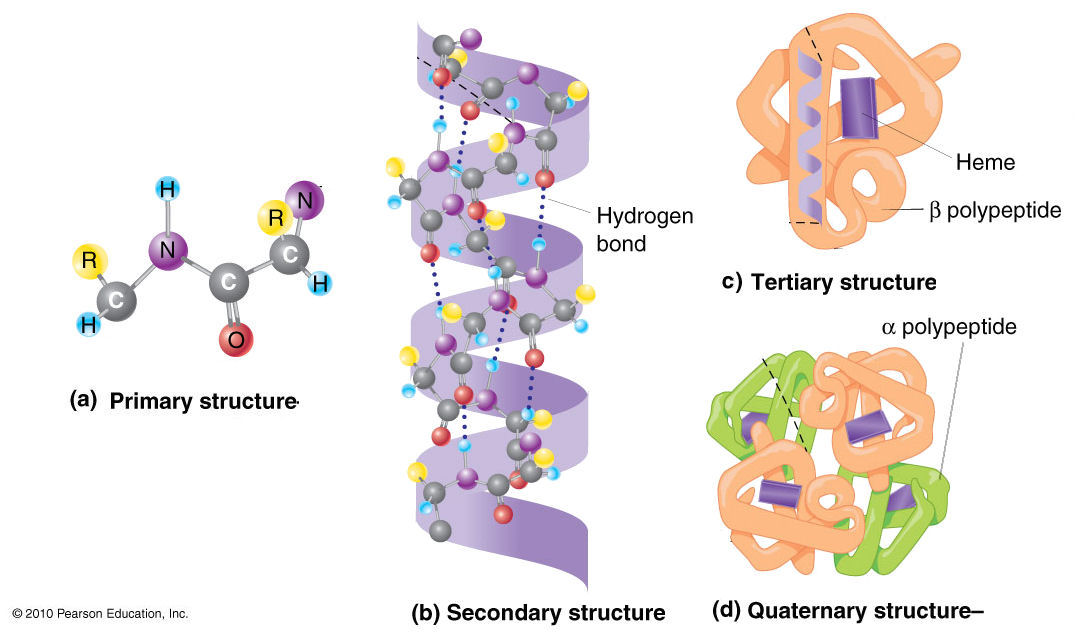
\includegraphics[width=10cm]{img/papers/protein_structure}
		\caption{Types of protein structures. Source: \cite{russell2002igenetics}.}
	\end{figure}
	
\end{frame}
%-------------------------------------------------------
%-------------------------------------------------------

%-------------------------------------------------------
%-------------------------------------------------------
\begin{frame}{Numbers}{}

	\begin{block}{}
		Protein structures are complex systems with several tens, hundreds and \textbf{thounsand} of residues (amino acids).	
	\end{block}	

	\begin{block}{}
		Only about \textbf{1\%} of the total number of sequenced proteins has experimentally determined \cite{rangwala2011introduction}.
	\end{block}	

\end{frame}
%-------------------------------------------------------
%-------------------------------------------------------

\subsection{Motivation}

%-------------------------------------------------------
%-------------------------------------------------------
\begin{frame}{Motivation}{}	

\begin{block}{}
	Is one of the most used task in Bioinformatics \cite{o2010visualization, mura2010introduction}.
\end{block}	
\pause
\begin{block}{}
	Ligand-binding pockets or other details in macromolecular assemblies helps to elucidate the	relationship between protein structure and function \cite{reynolds2018ezmol}.
\end{block}
\pause
\begin{block}{}
	Interactive visualization of large molecular structures can now be achieved via web-based 3D, It is not restricted to stand alone applications \cite{wang2020icn3d}.
\end{block}

\end{frame}
%-------------------------------------------------------
%-------------------------------------------------------

\subsection{Problem}
%-------------------------------------------------------
%-------------------------------------------------------
\begin{frame}{Problem}{}
	
\begin{block}{}
	There is not a robust Web-based tool for protein visualization. The current applications are in development:
	\begin{itemize}
		\item They have bugs.
		\item They doesn't have all the functionality like stand-alone applications. 
		\item They are not easy to use.
	\end{itemize}
\end{block}
	
\end{frame}
%-------------------------------------------------------
%-------------------------------------------------------


%%%%%%%%%%%%%%%%%%%%%%%%%%%%%%%%%%%%%%%%%%%%%%%%%%%%%%%%%%%%%%%%%%%%%%%%%%%%%%%%%%%%%%%%%%%%%%%%%%%%%%%%%%%%%%%%
%%%%%%%%%%%%%%%%%%%%%%%%%%%%%%%%%%%%%%%%%%%%%%%%%%%%%%%%%%%%%%%%%%%%%%%%%%%%%%%%%%%%%%
\section{Related work}
%%%%%%%%%%%%%%%%%%%%%%%%%%%%%%%%%%%%%%%%%%%%%%%%%%%%%%%%%%%%%%%%%%%%%%%%%%%%%%%%%%%%%%%%%%%%%%%%%%%%%%%%%%%%%%%%
%%%%%%%%%%%%%%%%%%%%%%%%%%%%%%%%%%%%%%%%%%%%%%%%%%%%%%%%%%%%%%%%%%%%%%%%%%%%%%%%%%%%%%

%-------------------------------------------------------
%-------------------------------------------------------
\begin{frame}{Related work}{Jolecule}	
	\begin{figure}
		\centering
		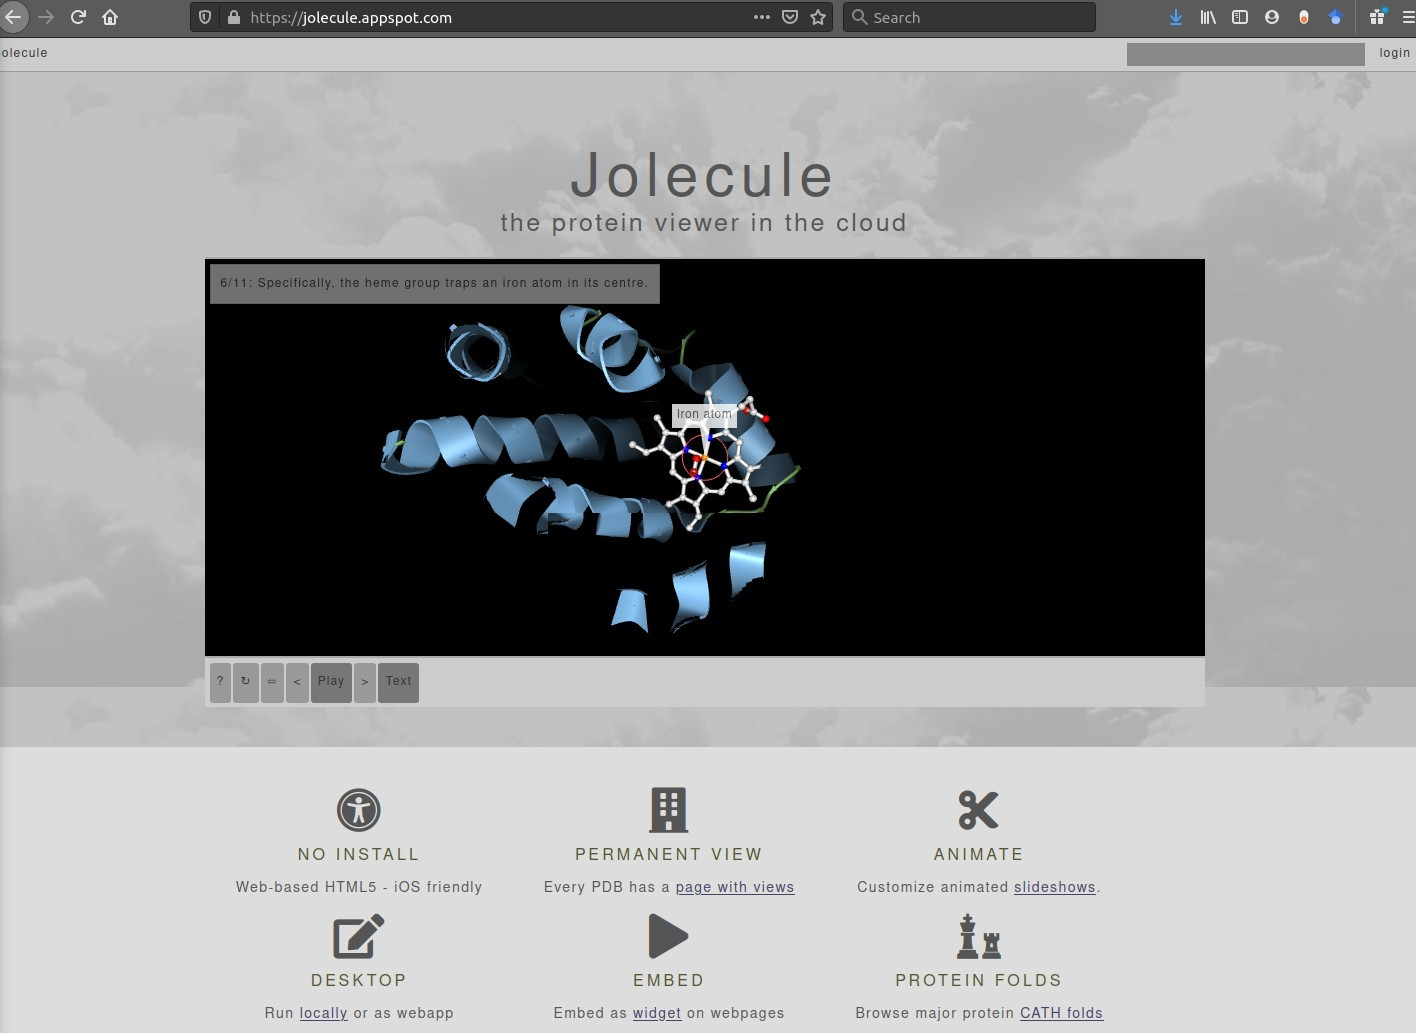
\includegraphics[width=8cm]{img/argosmol/state_art1}
		\caption{Web page of Jolecule.}
	\end{figure}
\end{frame}
%-------------------------------------------------------
%-------------------------------------------------------

%-------------------------------------------------------
%-------------------------------------------------------
\begin{frame}{Related work}{NGL}	
	\begin{figure}
		\centering
		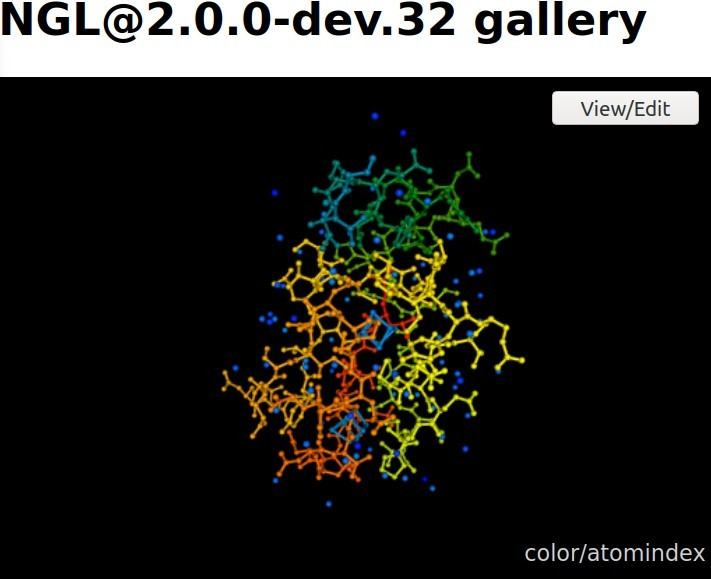
\includegraphics[width=8cm]{img/argosmol/state_art2}
		\caption{Web page of NGL \cite{rose2015ngl}.}
	\end{figure}
\end{frame}
%-------------------------------------------------------
%-------------------------------------------------------

%-------------------------------------------------------
%-------------------------------------------------------
\begin{frame}{Related work}{EzMol}	
	\begin{figure}
		\centering
		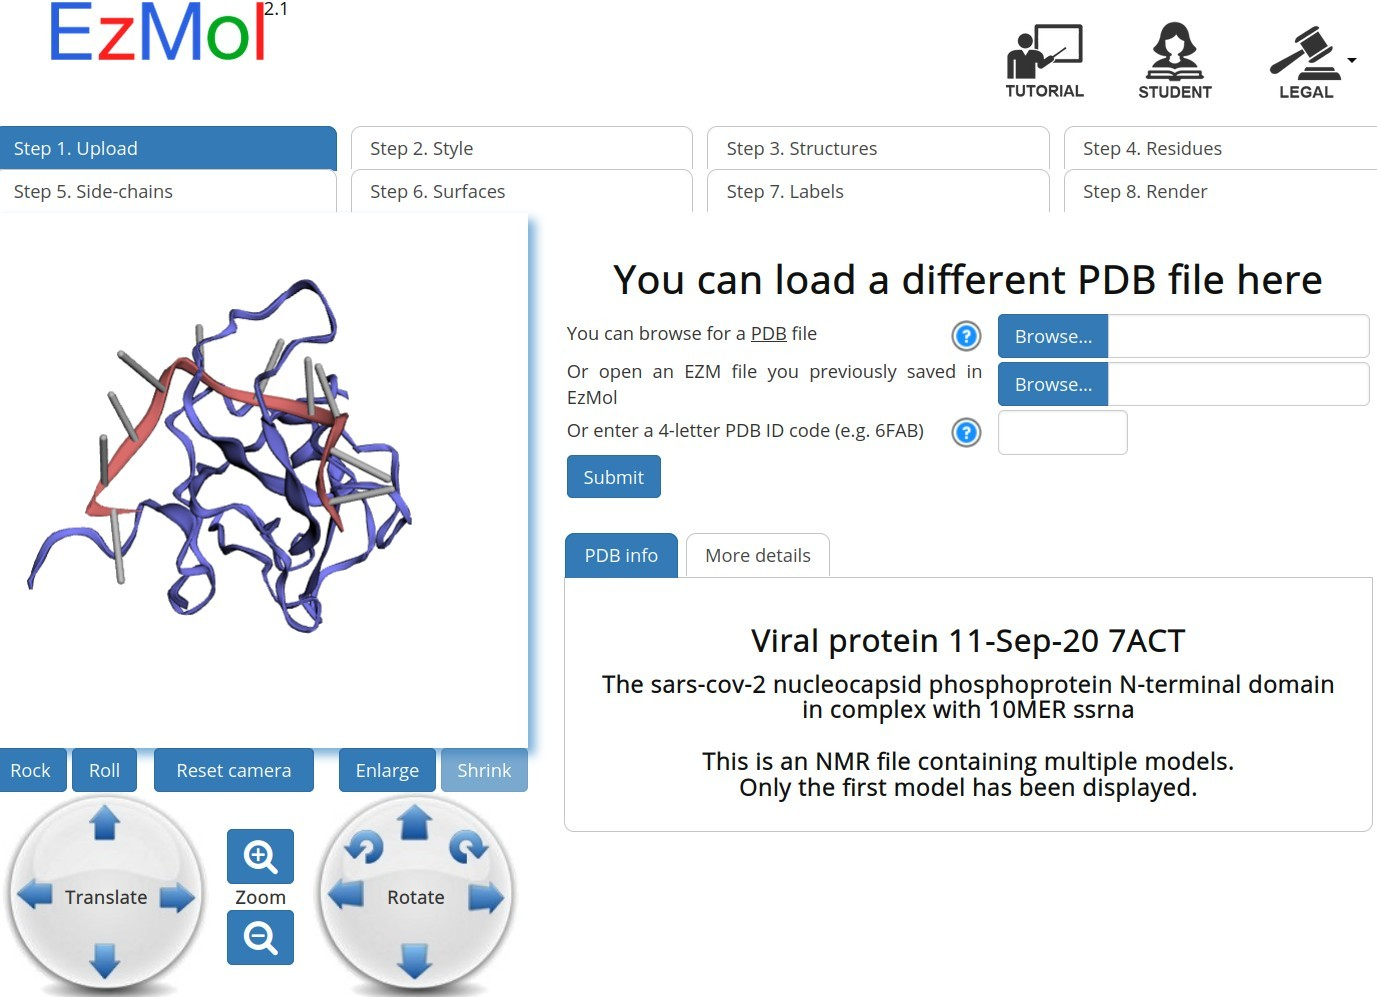
\includegraphics[width=8cm]{img/argosmol/state_art3}
		\caption{Web page of EzMol \cite{reynolds2018ezmol}.}
	\end{figure}
\end{frame}
%-------------------------------------------------------
%-------------------------------------------------------

%-------------------------------------------------------
%-------------------------------------------------------
\begin{frame}{Related work}{iCn3D}	
	\begin{figure}
		\centering
		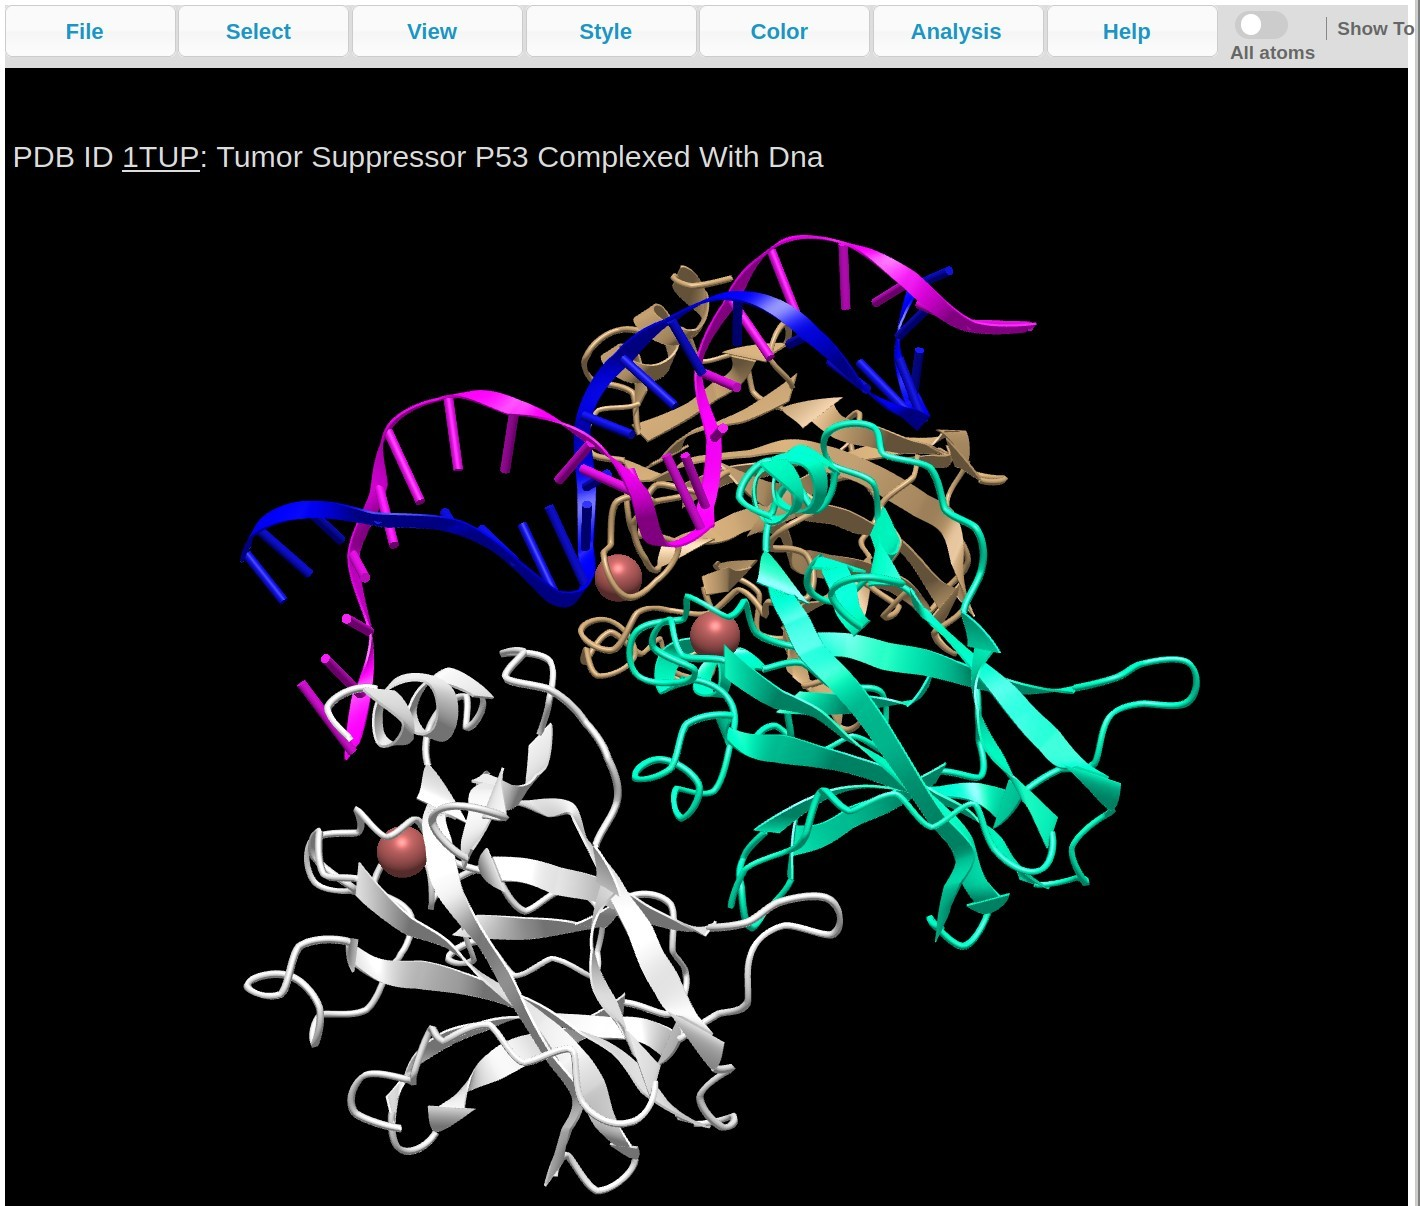
\includegraphics[width=8cm]{img/argosmol/state_art4}
		\caption{Web page of iCn3D \cite{wang2020icn3d}.}
	\end{figure}
\end{frame}
%-------------------------------------------------------
%-------------------------------------------------------

%-------------------------------------------------------
%-------------------------------------------------------
%\begin{frame}{Related work}{Web3DMol}	%
%	\begin{figure}
%		\centering
%		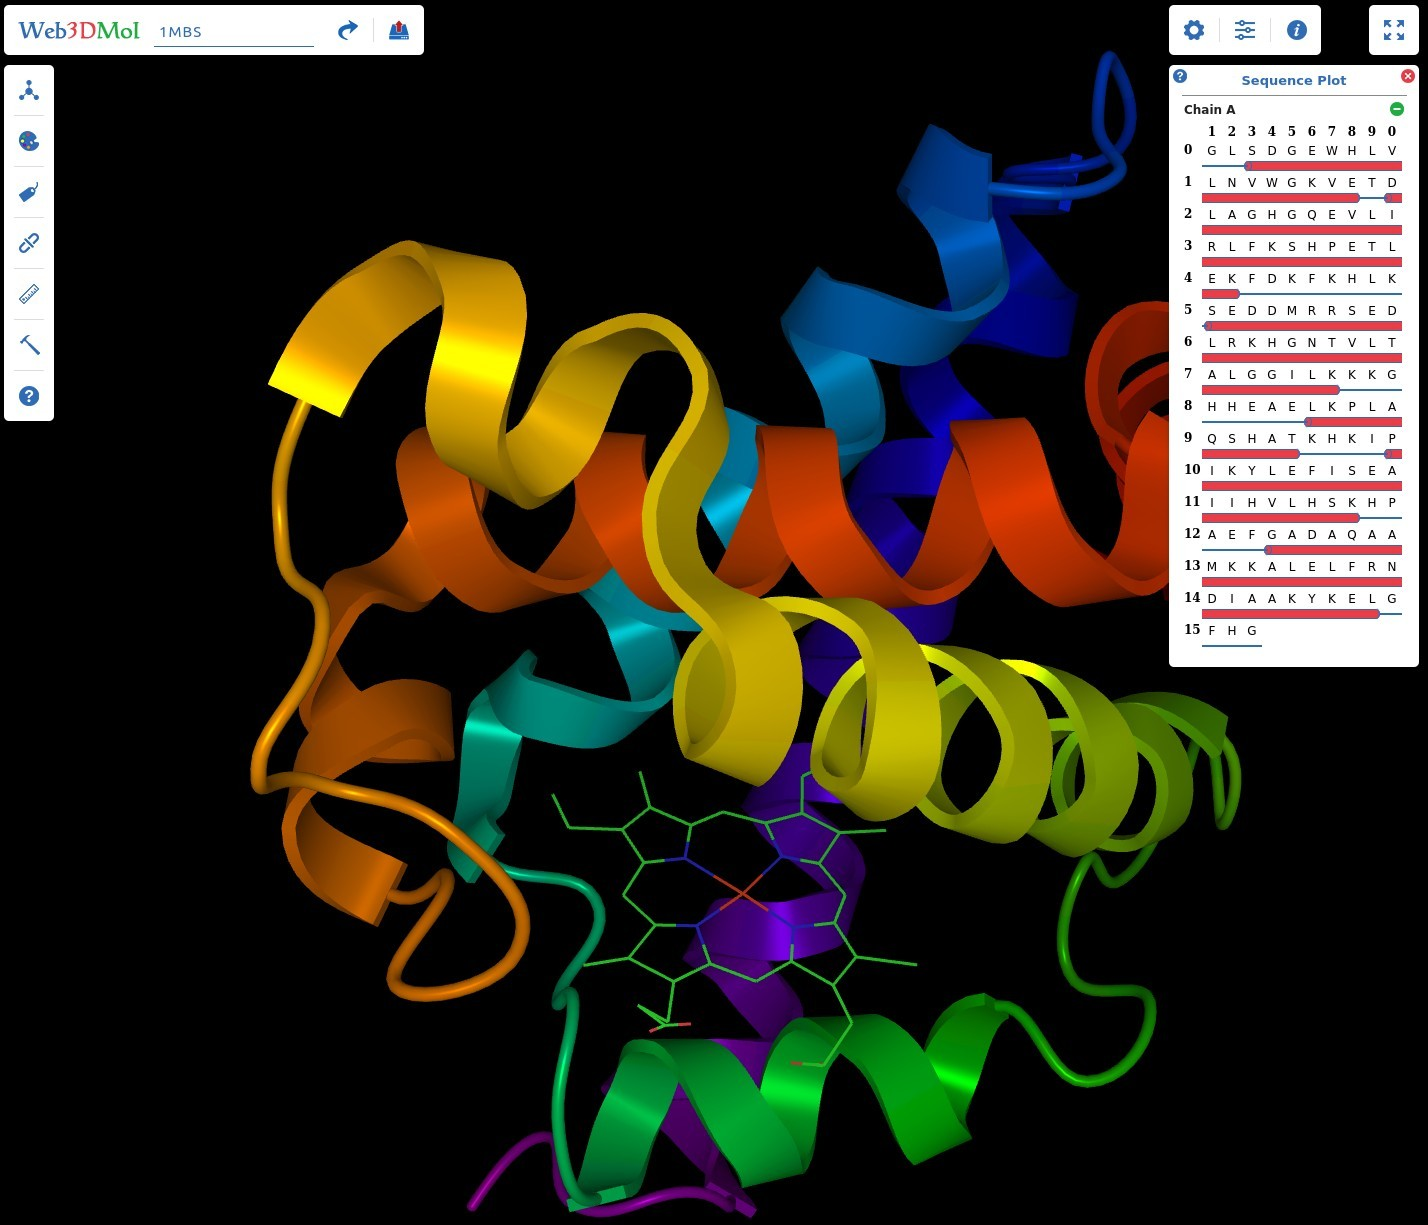
\includegraphics[width=8cm]{img/argosmol/state_art5}
%		\caption{Web page of Web3DMol \cite{shi2017web3dmol}.}
%	\end{figure}
%\end{frame}
%-------------------------------------------------------
%-------------------------------------------------------



%%%%%%%%%%%%%%%%%%%%%%%%%%%%%%%%%%%%%%%%%%%%%%%%%%%%%%%%%%%%%%%%%%%%%%%%%%%%%%%%%%%%%%%%%%%%%%%%%%%%%%%%%%%%%%%%
%%%%%%%%%%%%%%%%%%%%%%%%%%%%%%%%%%%%%%%%%%%%%%%%%%%%%%%%%%%%%%%%%%%%%%%%%%%%%%%%%%%%%%
\section{Proposal}
%%%%%%%%%%%%%%%%%%%%%%%%%%%%%%%%%%%%%%%%%%%%%%%%%%%%%%%%%%%%%%%%%%%%%%%%%%%%%%%%%%%%%%%%%%%%%%%%%%%%%%%%%%%%%%%%
%%%%%%%%%%%%%%%%%%%%%%%%%%%%%%%%%%%%%%%%%%%%%%%%%%%%%%%%%%%%%%%%%%%%%%%%%%%%%%%%%%%%%%

%%%%%%%%%%%%%%%%%%%%%%%%%%%%%%%%%%%%%%%%%%%%%%%%%%%%%%%%%%%%%%%%%%%%%%%%%%%%%%%%%%%%%%%%%%%%%%%%%%%%%%%%%%%%%%%%
%%%%%%%%%%%%%%%%%%%%%%%%%%%%%%%%%%%%%%%%%%%%%%%%%%%%%%%%%%%%%%%%%%%%%%%%%%%%%%%%%%%%%%
\subsection{ArgosMol}
%%%%%%%%%%%%%%%%%%%%%%%%%%%%%%%%%%%%%%%%%%%%%%%%%%%%%%%%%%%%%%%%%%%%%%%%%%%%%%%%%%%%%%%%%%%%%%%%%%%%%%%%%%%%%%%%
%%%%%%%%%%%%%%%%%%%%%%%%%%%%%%%%%%%%%%%%%%%%%%%%%%%%%%%%%%%%%%%%%%%%%%%%%%%%%%%%%%%%%%

%-------------------------------------------------------
%-------------------------------------------------------
\begin{frame}{ArgosMol}{}	
	\begin{figure}
		\centering
		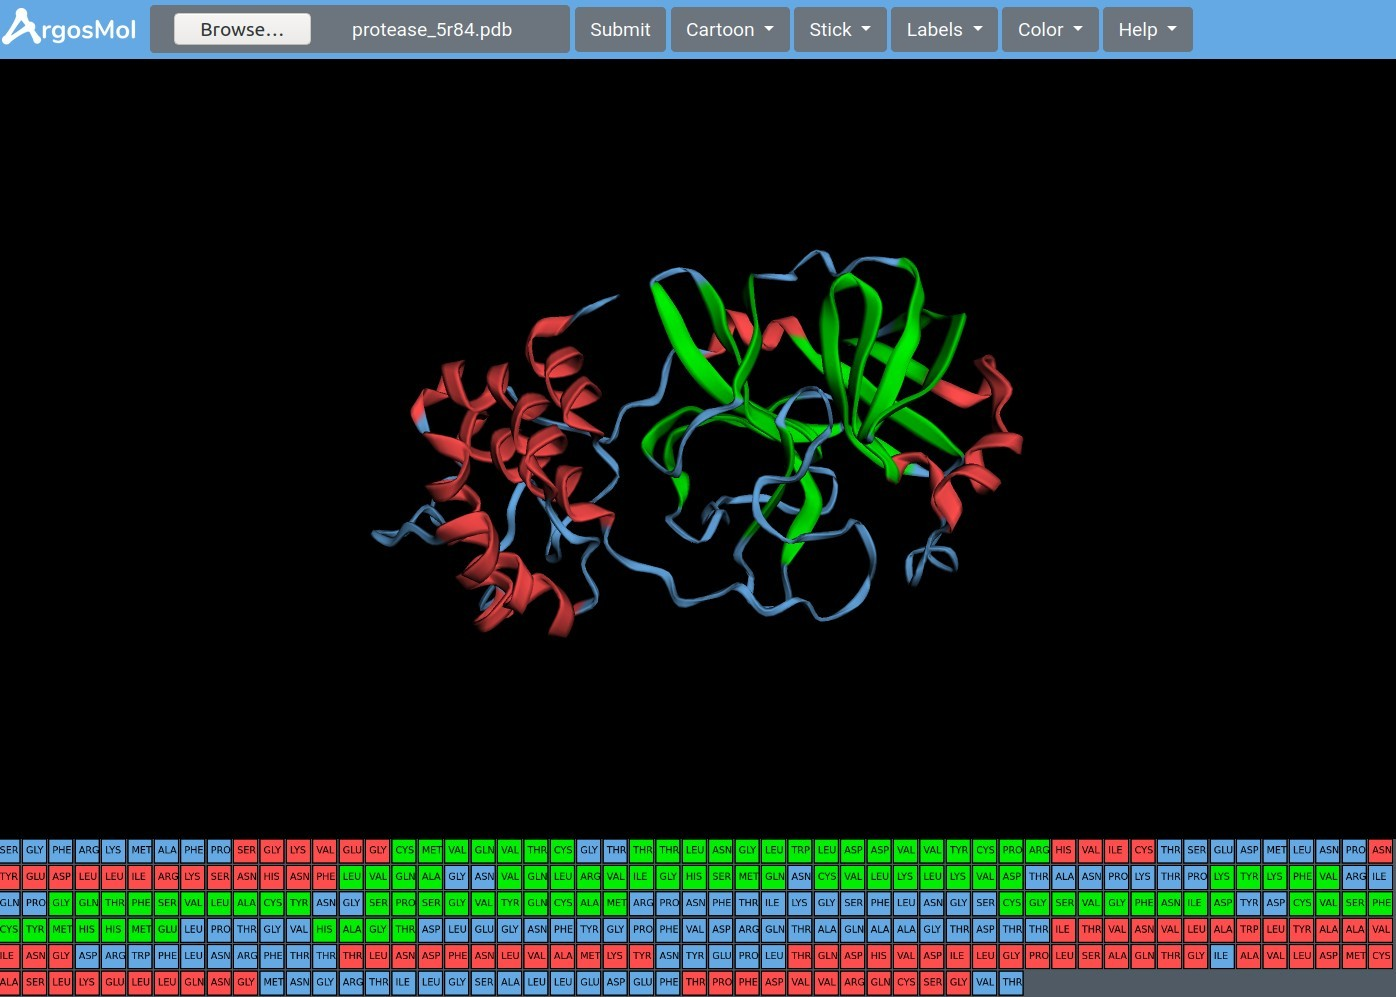
\includegraphics[width=8cm]{img/argosmol/argos1}
		\caption{Web page of ArgosMol \chref{http://134.209.44.160/argosmol/protein_interaction.php}{Enlace}.}
	\end{figure}
\end{frame}
%-------------------------------------------------------
%-------------------------------------------------------

%-------------------------------------------------------
%-------------------------------------------------------
\begin{frame}{ArgosMol}{Visualization}	
	\begin{figure}[h]
		\centering
		\begin{multicols}{2}
			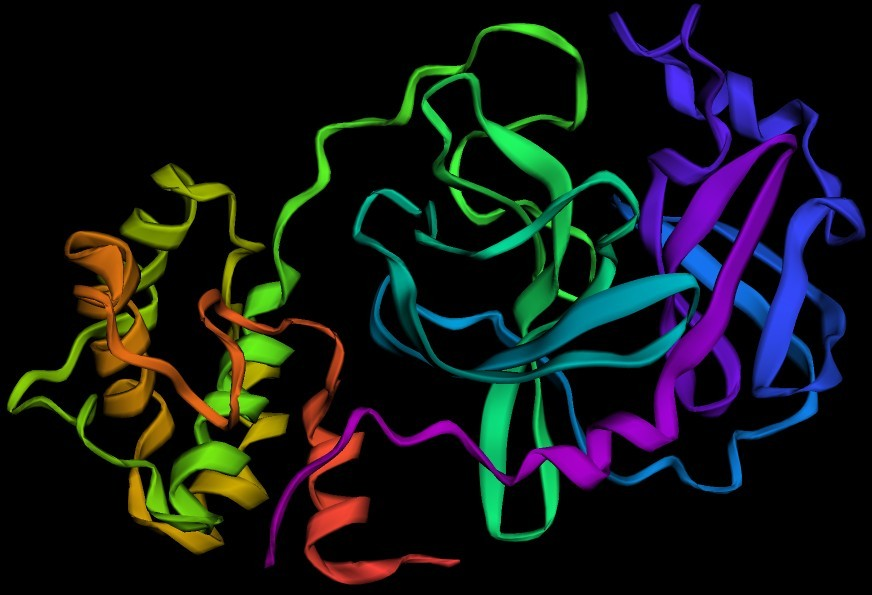
\includegraphics[width=5cm,height=3cm]{img/argosmol/argos2}\par 
			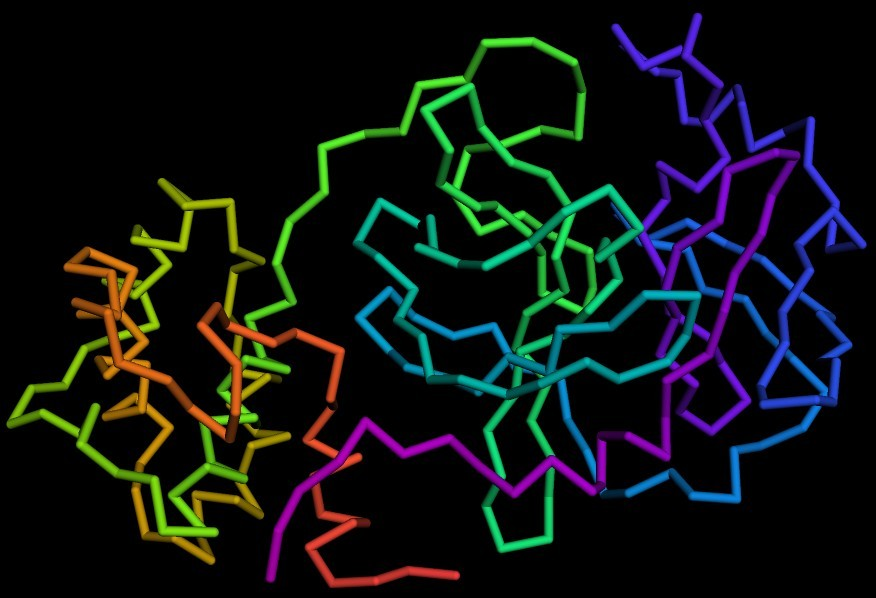
\includegraphics[width=5cm,height=3cm]{img/argosmol/argos3}\par 
			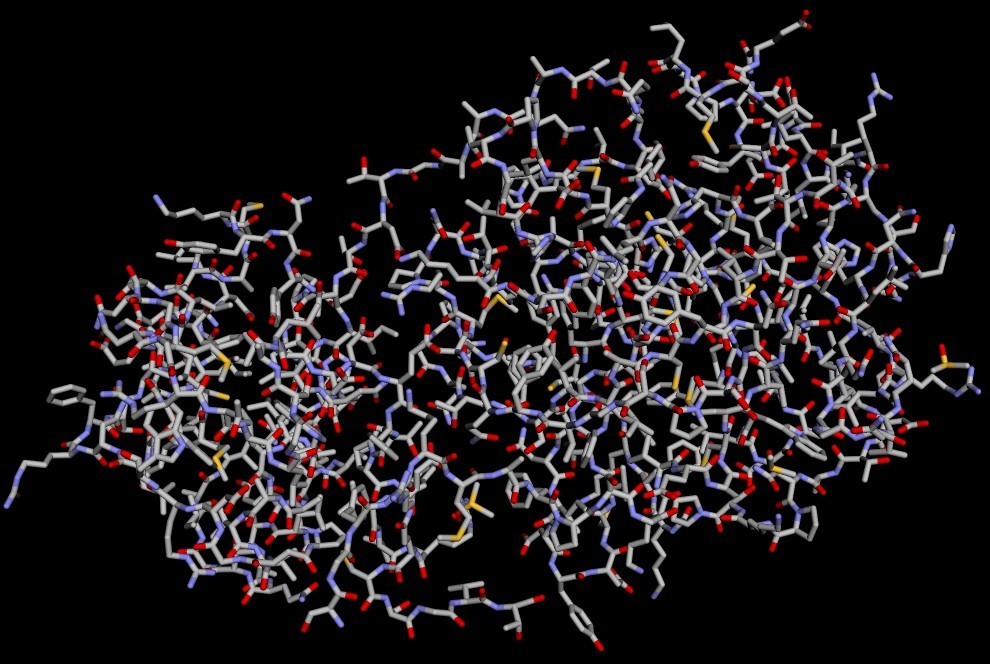
\includegraphics[width=5cm,height=3cm]{img/argosmol/argos4}\par 
			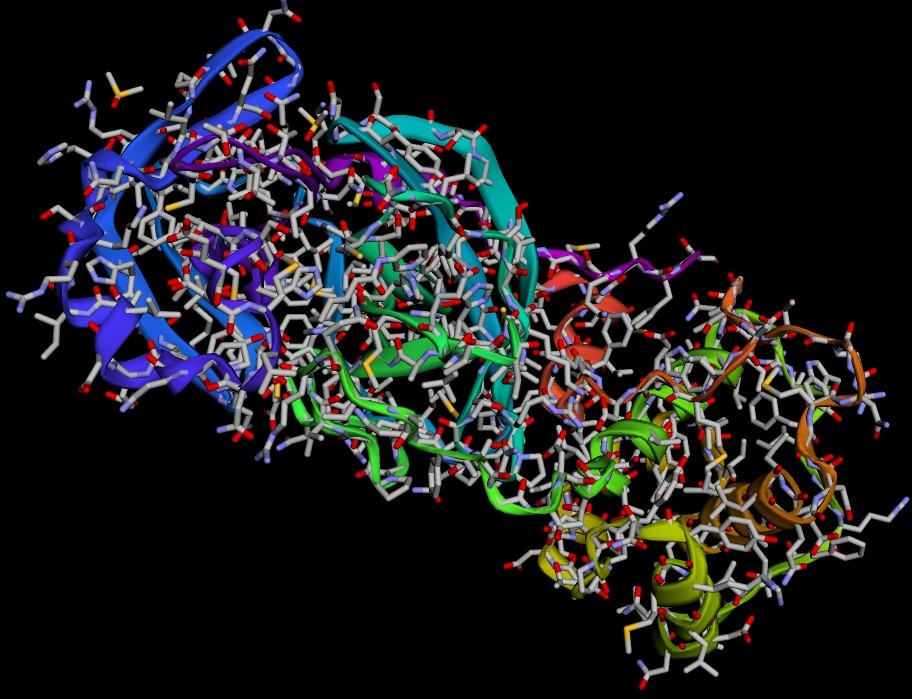
\includegraphics[width=5cm,height=3cm]{img/argosmol/argos5}\par 
		\end{multicols}
		\caption{Visualization in ArgosMol.}
		\label{fig:protein_1}
	\end{figure}
\end{frame}
%-------------------------------------------------------
%-------------------------------------------------------


%-------------------------------------------------------
%-------------------------------------------------------
\begin{frame}{ArgosMol}{Colors}	
	\begin{figure}[h]
		\centering
		\begin{multicols}{2}
			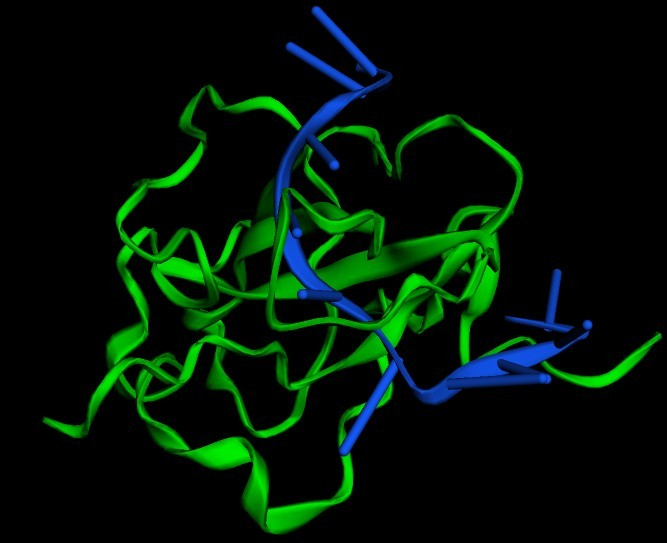
\includegraphics[width=5cm,height=3cm]{img/argosmol/argos6}\par 
			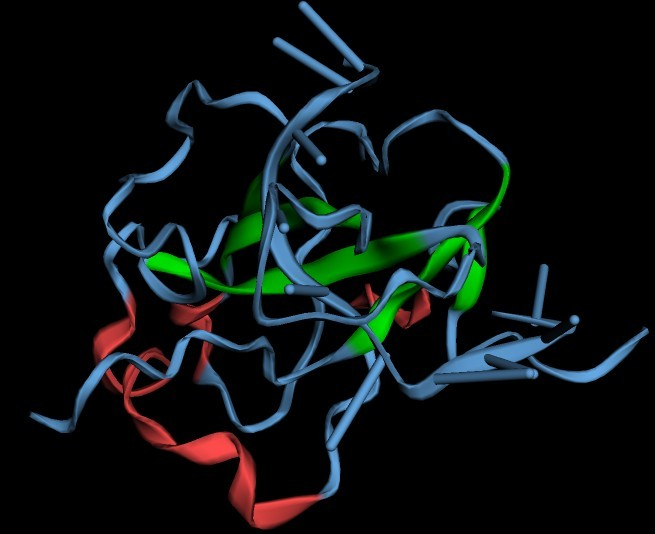
\includegraphics[width=5cm,height=3cm]{img/argosmol/argos7}\par 
			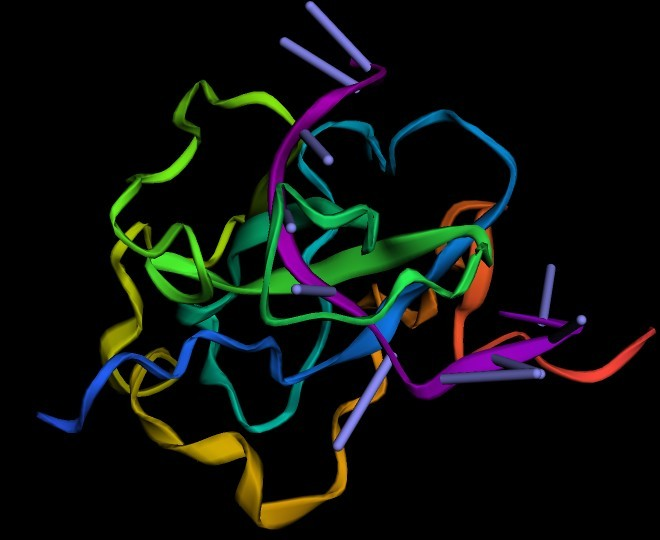
\includegraphics[width=5cm,height=3cm]{img/argosmol/argos8}\par 
			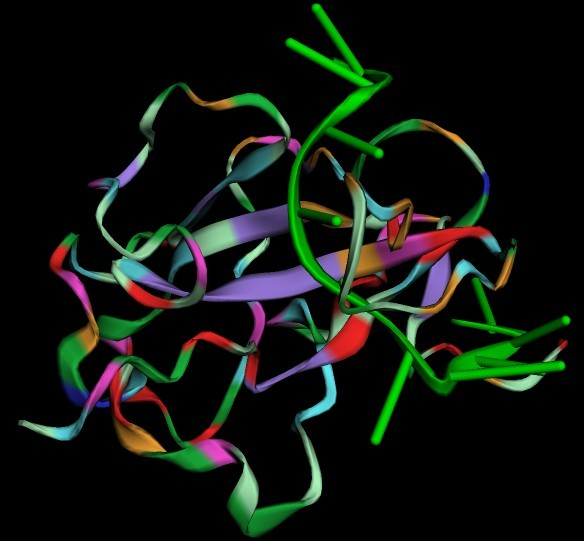
\includegraphics[width=5cm,height=3cm]{img/argosmol/argos9}\par 
		\end{multicols}
		\caption{Colors in ArgosMol.}
		\label{fig:protein_1}
	\end{figure}
\end{frame}
%-------------------------------------------------------
%-------------------------------------------------------

%-------------------------------------------------------
%-------------------------------------------------------
\begin{frame}{ArgosMol}{Model and sequence}	
	\begin{figure}
		\centering
		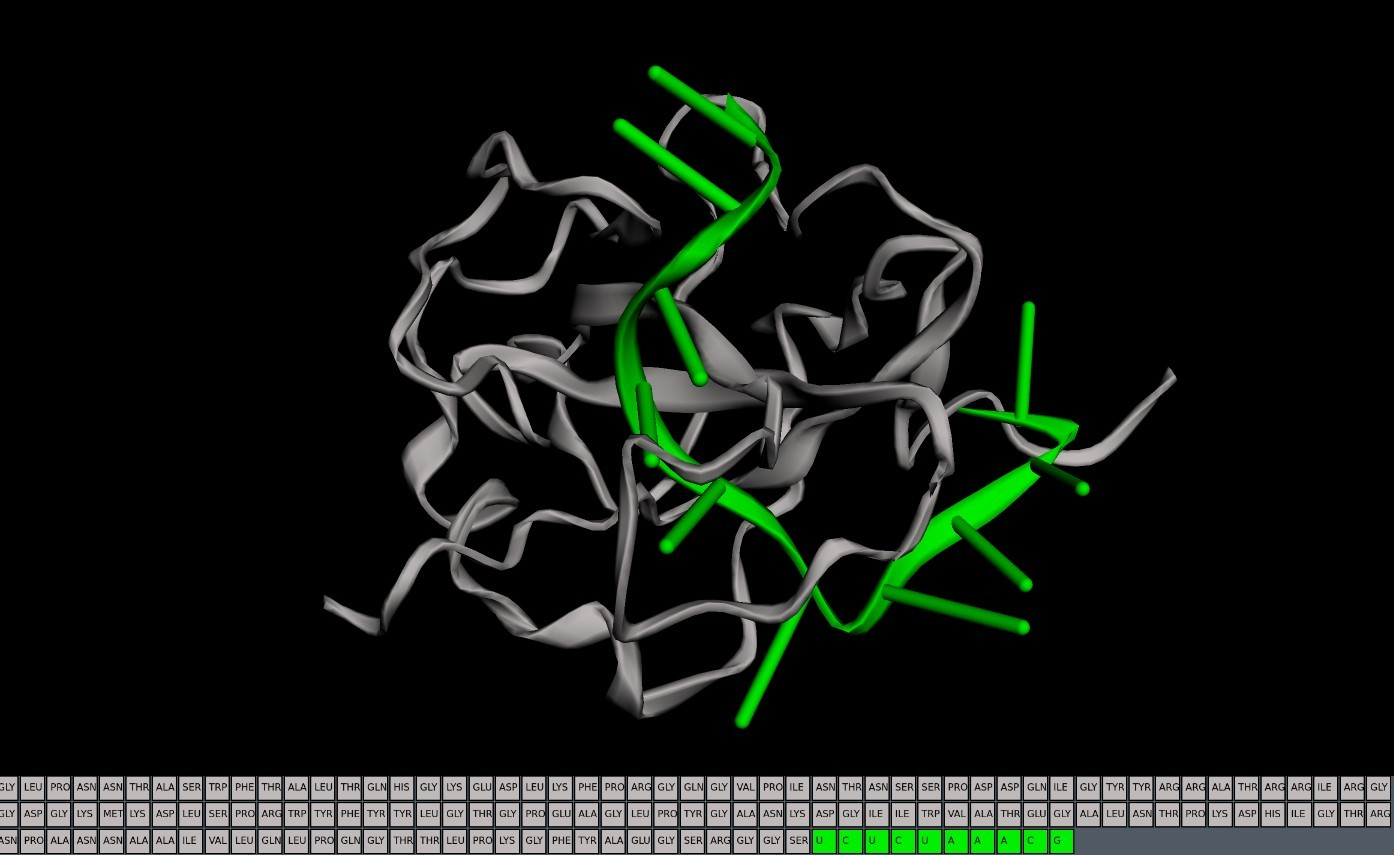
\includegraphics[width=10cm]{img/argosmol/argos10}
		\caption{Relation between the model and the sequence in ArgosMol.}
	\end{figure}
\end{frame}
%-------------------------------------------------------
%-------------------------------------------------------

%%%%%%%%%%%%%%%%%%%%%%%%%%%%%%%%%%%%%%%%%%%%%%%%%%%%%%%%%%%%%%%%%%%%%%%%%%%%%%%%%%%%%%%%%%%%%%%%%%%%%%%%%%%%%%%%
%%%%%%%%%%%%%%%%%%%%%%%%%%%%%%%%%%%%%%%%%%%%%%%%%%%%%%%%%%%%%%%%%%%%%%%%%%%%%%%%%%%%%%
\section{Conclusions}
%%%%%%%%%%%%%%%%%%%%%%%%%%%%%%%%%%%%%%%%%%%%%%%%%%%%%%%%%%%%%%%%%%%%%%%%%%%%%%%%%%%%%%%%%%%%%%%%%%%%%%%%%%%%%%%%
%%%%%%%%%%%%%%%%%%%%%%%%%%%%%%%%%%%%%%%%%%%%%%%%%%%%%%%%%%%%%%%%%%%%%%%%%%%%%%%%%%%%%%
%-------------------------------------------------------
%-------------------------------------------------------
\begin{frame}{Conclusions}{}	

	\begin{block}{}
		ArgosMol is an alternative to stand-alone applications that requiere instalation.
	\end{block}

	\begin{block}{}
		ArgosMol is part of a small number of Web-based tools for protein viosualization. Nevertheleses, ArgosMol improve the usability and the relation between the model and sequence.
	\end{block}

	\begin{block}{}
		In future version of ArgosMol, we will include protein structure prediction.
	\end{block}

\end{frame}
%-------------------------------------------------------
%-------------------------------------------------------

%-------------------------------------------------------
%-------------------------------------------------------
\begin{frame}[allowframebreaks]
	\frametitle{References}
	%\bibliographystyle{amsalpha}
	\bibliographystyle{IEEEtran}
	\bibliography{bibliography.bib}
\end{frame}
%-------------------------------------------------------
%-------------------------------------------------------


%-------------------------------------------------------
%-------------------------------------------------------
\if\mycmd1 % MY THEME
\1{
	{\1
		\begin{frame}[plain,noframenumbering]
			%\finalpage{Thank you}
			\begin{figure}[]
				\centering
				
\includegraphics[width=\textwidth,height=0.7\textheight,keepaspectratio]{img/question.png}
				%\label{img:mot2}
				%\caption{Image example in 2 gray levels.}
			\end{figure}
	\end{frame}}
	\else % CS THEME
	\begin{frame}{Questions?}
		\begin{figure}[]
			\centering
			
\includegraphics[width=\textwidth,height=0.7\textheight,keepaspectratio]{img/question.png}
			%\label{img:mot2}
			%\caption{Image example in 2 gray levels.}
		\end{figure}
		
	\end{frame}
	\fi
	%-------------------------------------------------------
	%-------------------------------------------------------
	

\end{document}